\documentclass[a4paper,12pt]{article}

\usepackage[utf8]{inputenc}
\usepackage[french]{babel}
\usepackage{fullpage,url,graphicx,alltt}

\newcommand{\mlpost}{\textsc{Mlpost}}
\newcommand{\gmlpost}{\textsc{GMlpost}}
\newcommand{\meta}{\textsc{Metapost}}

\title{\huge{TER Stage : ~\\
  Implémentation d'une bibliothèque de diagrammes pour \mlpost}}
\author{ Guillaume Von Tokarski et Julien Robert}

\begin{document}
\maketitle

\begin{center}M1 Informatique, Université Paris Sud XI\end{center}
\newpage
\tableofcontents
\newpage
\section{Introduction}

\subsection{Présentation de \mlpost}
\mlpost\ est une bibliothèque OCaml développée au sein du projet Proval de l’INRIA Saclay – Île-de-France, permettant la réalisation de dessins scientifiques destinés à être inclus dans des documents \LaTeX \cite{mlpost}.

\subsubsection{Motivations}
Dans un cadre scientifique, il est très souvent nécessaire d'inclure des figures aux documents (cours, articles). Il existe bien sûr de nombreux éditeurs graphiques, mais la conception de figures complexes s'avère longue et nuit à l'homogénéité du tout. 
\bigskip 


Une façon très commune de rédiger ces documents est d'utiliser \LaTeX. \LaTeX\ et \meta\ permettent la création de figures, mais ces langages sont difficiles d'utilisation, notamment avec des messages d'erreurs compliqués. Il doit également être possible d'ajouter des éléments de \LaTeX\ ($\Pi$, $\Sigma$ ...) à la figure, et de garder une homogénéité du document, ce qui s'avère impossible avec des éditeurs graphiques comme Dia ou Gimp. 
\bigskip

Les concepteurs ont choisi d'interfacer \meta\ avec OCaml. Un langage comme OCaml permet de résoudre les erreurs plus aisément que \meta. OCaml bénéficie d'arguments optionnels, très pratiques dans la conception d'une librairie graphique. 

Enfin il est important de préciser qu'une figure \mlpost\ peut être utilisée comme la vue du résultat d'un calcul ou d'un algorithme. On pourra par exemple calculer un arbre couvrant d'un graphe, et le représenter sous forme d'arbre \mlpost\ dans le même programme.

\subsubsection{Structure de \mlpost}
\mlpost\ est constitué de nombreux modules open sources séparés en quatre catégories:
\begin{itemize}
\item les interfaces des types basiques de \meta\ (Command,Num,Point,Path,Picture...)
\item les composants graphiques avancés (Box,Shapes,Arrow...) 
\item les extensions (Tree,Histogram,Diag,Plot...)
\item les modules de génération de \meta
\end{itemize}

Pour simplifier les choses, on peut dire qu'une figure est une liste de commandes (module Command) qui sera passée aux modules de génération de \meta.


\subsubsection{Exemples}
L'exemple ci-dessous est une simple utilisation de boîte avec \mlpost. On notera l'utilisation du symbole mathématique $\pi$ qui se fait aisément en conservant l'homogénéité du tout, ainsi que la concision du code pour générer la boîte.
\bigskip 

\begin{minipage}{0.7\linewidth}
  \begin{alltt}
    let simple_block =
    let b = Box.hblock ~pos:`Bot 
    [Box.tex "a"; Box.tex "A"; Box.tex "1"; 
     Box.tex "$\\pi$"] 
    in
    Box.draw b
  \end{alltt}
\end{minipage}
\begin{minipage}{0.3\linewidth}
  \begin{center}
    \includegraphics[scale=2]{simple_block.mps}
  \end{center}
\end{minipage}


Un exemple légèrement plus compliqué dans lequel on utilise des arguments optionnels pour mieux personnaliser la figure.
\bigskip 

\begin{minipage}{0.7\linewidth}
  \begin{alltt}
    let traffic =
    let two = Num.bp 2. in
    let b = 
    vbox ~fill:black ~padding:(Num.bp 3.) ~dx:two ~dy:two
    [ tex ~style:Circle ~fill:red "R";
      tex ~style:Circle ~fill:yellow "Y";
      tex ~style:Circle ~fill:green "G"; ]
    in
    draw b
  \end{alltt}
\end{minipage}
\begin{minipage}{0.3\linewidth}
  \begin{center}
    \includegraphics[scale=2]{traffic.mps}
  \end{center}
\end{minipage}


Un dernier exemple plus compliqué utilisant les module Path, Point et Pen pour dessiner un rubik's cube. Cette figure étant le résultat d'un calcul, on voit bien à quel point il serait facile de changer certains paramètres pour la modifier.
\bigskip 

\begin{minipage}{0.7\linewidth}
  \begin{alltt}
    let alpha = atan 1.
    let beta = atan 1. /. 2. 
    let mag = 10.
    
    let proj x y z = 
    mag *. float (x - y) *. cos alpha, 
    mag *. (float (x + y) *. sin alpha *. sin beta +. float z *. cos beta)
    
    let pen = Pen.scale (bp 2.5) Pen.default
  
    let square color p i j =
    let pt i j = let x,y = p i j in 
    Point.pt (bp x, bp y) in
    let points = [pt i j; pt (i+1) j; 
      pt (i+1) (j+1); pt i (j+1)] in
    let path = pathp ~style:jLine 
    ~cycle:jLine points in
    seq [fill ~color path; Command.draw ~pen path]
    
    let right = square Color.orange (fun i j -> proj i 0 j)
    let up = square Color.yellow (fun i j -> proj i j 3)
    let left = square Color.green (fun i j -> proj 0 (3 - i) j)
    
    let rubik = 
    seq [iter 0 2 (fun i -> iter 0 2 (right i));
      iter 0 2 (fun i -> iter 0 2 (up i));
      iter 0 2 (fun i -> iter 0 2 (left i));]
  \end{alltt}
\end{minipage}
\begin{minipage}{0.3\linewidth}
  \begin{center}
    \includegraphics[scale=3]{rubik.mps}
  \end{center}
\end{minipage}

\subsection{Notre TER}
Le sujet du stage était à l'origine \textit{Implémentation d'une
  bibliothèque de diagrammes pour \mlpost}. Il s'agissait de réaliser une extension de \mlpost, sans bien sûr avoir à modifier ce qui était déjà présent. Nous avons donc dû d'abord maîtriser très vite l'API.
Pour ce stage, il fallait bien sûr que notre API soit claire, dans les choix de types, de noms de fonctions et d'arguments (surtout optionnels), et qu'elle soit accompagnée d'une documentation (conçue avec \textsc{OCamldoc}).

Dans la deuxième partie du stage, notre encadrant nous a proposé de modifier le module Tree et d'implémenter une interface graphique pour \mlpost.

\subsubsection{Modules au dessus de \mlpost}
Nous avons travaillé sur cinq modules. 
Sur ces cinq modules, nous en avons créé trois (Histogram,Radar,Legend), enrichi un (Path), et modifié un autre (Tree).
Nos trois modules sont des modules \og haut niveau\fg\ qui n'ont nécessité aucune modification du noyau de \mlpost. 
\subsubsection{Interface Graphique}
\gmlpost\ est une interface graphique de \mlpost\ permettant l'édition de figures \mlpost\ avec un gain de temps de praticité. Sa conception nous a permis de devenir familier avec \textsc{lablgtk2} (et donc \textsc{gkt2} par extension) et d'utiliser à nouveau l'outil \textsc{OCamllex}.

\section{Modules \mlpost}

\subsection{Histogram}
Il existe trois types d'histogrammes:
\begin{itemize}
\item simple,
\item comparatif,
\item cumulatif.
\end{itemize}
\bigskip 

Le c\oe ur du module est la fonction  \texttt{hist}. Cette fonction est nécessaire car elle permet de factoriser une grande quantité de code commun à chaque type d'histogramme. Elle permet la création d'un ensemble de boîtes avec leurs labels. La fonction \texttt{hist} renvoie une Command, qui est utilisée par les fonctions -- simple, compare, stack -- couplée au dessin d'un repère grâce au module Plot.
Concrètement, un histogramme est une \texttt{hbox}, un alignement horizontal de boîtes. Chaque boîte contient une \texttt{vbox}, un alignement vertical de boîtes. Ceci forme une sorte de matrice, où chaque élément est un morceau d'histogramme.

\subsubsection{Simple:}
Un histogramme classique construit à partir d'une liste de nombres
flottants.
\begin{alltt}
  val simple :
  ?width:Num.t ->
  ?height:Num.t ->
  ?padding:Num.t ->
  ?fill:Color.t list ->
  ?perspective: bool ->
  ?hcaption:Picture.t ->
  ?vcaption:Picture.t ->
  ?histlabel:[> `Bot | `Center | `Top ] * Picture.t labels ->
  ?vlabel:Plot.labels ->
  ?hlabel:Picture.t list -> 
  float list -> Command.t
\end{alltt}

\bigskip

\begin{minipage}{0.5\linewidth}
  \begin{alltt}
    let hist1 = Hist.simple
    [3.;1.;6.]
  \end{alltt}

  Utilisation très simple de \texttt{simple} pour trois valeurs. On spécifie la taille totale de la figure. La construction de cet histogramme nécessite un appel à la fonction \texttt{hist} et l'ajout d'un repère. Un histogramme simple est une matrice où chaque colonne est un seul élément, c'est-à-dire une \texttt{hbox} dont chaque sous boîte contient une \texttt{vbox} qui contient un seul élément.
\end{minipage}
\begin{minipage}{0.5\linewidth}
  \begin{center}
    \includegraphics[scale=1.]{hist1.mps}
  \end{center}
\end{minipage}

\subsubsection{Comparatif :} 
Un histogramme comparatif construit à partir d'une liste. Cette liste
contient des listes de nombres flottants, chacune étant un histogramme.
\begin{alltt}
  val compare :
  ?width:Num.t ->
  ?height:Num.t ->
  ?padding:Num.t ->
  ?fill:Color.t list ->
  ?perspective: bool ->
  ?hcaption:Picture.t ->
  ?vcaption:Picture.t ->
  ?histlabel:[> `Bot | `Center | `Top ] * Picture.t list labels ->
  ?vlabel:Plot.labels ->
  ?hlabel:Picture.t list ->
  float list list -> Command.t
\end{alltt}

\bigskip

\begin{minipage}{0.5\linewidth}
  \begin{alltt}
    let hist2 = Hist.compare
    ~width:(bp 100.)
    ~height:(bp 200.)
    [[1.;5.;6.;5.;3.];
      [1.;2.;3.;6.;-1.]]
  \end{alltt}
  
  L'histogramme comparatif se construit ici après deux appels à \texttt{hist}. Ceci génère deux histogrammes \og simples \fg\, avec un padding entre les barres calculé pour mettre ces histogrammes côtes à côtes, et une légère translation pour le deuxième, puis le repère est calculé.
\end{minipage}
\begin{minipage}{0.5\linewidth}
\begin{center}
\includegraphics[scale=1.]{hist2.mps}
\end{center}
\end{minipage}

\subsubsection{Cumulatif :} 
Un histogramme cumulatif est construit avec la même signature que les histogrammes comparatifs. Cependant, chaque sous liste correspond cette fois à une barre cumulée.
\begin{alltt}
  val stack :
  ?width:Num.t ->
  ?height:Num.t ->
  ?padding:Num.t ->
  ?fill:Color.t list ->
  ?perspective: bool ->
  ?hcaption:Picture.t ->
  ?vcaption:Picture.t ->
  ?histlabel:[> `Bot | `Center | `Top ] * Picture.t list labels ->
  ?vlabel:Plot.labels ->
  ?hlabel:Picture.t list -> 
  float list list -> Command.t
\end{alltt}

\bigskip

\begin{minipage}{0.5\linewidth}
  \begin{alltt}
    let hist3 =
    let vlabel _ _ = None in
    Hist.stack 
    ~vlabel
    ~fill:[lightred;lightblue;
      lightyellow;lightgreen]
    [[4.;5.;5.;]; [8.;3.;1.]; [2.;8.;1.;4.];
      [1.5;3.5];[2.;2.;7.;1.]]
  \end{alltt}
  
  Cette figure est construite à partir d'un seul appel de la fonction \texttt{hist}. Contrairement à l'histogramme \og simple \fg, chaque colonne est désormais constituée de plusieurs boîtes, c'est à dire chaque \texttt{vbox} contient désormais plusieurs boîtes. L'histogramme \og simple \fg\ est donc un cas particulier de l'histogramme \og cumulatif \fg.
\end{minipage}
\begin{minipage}{0.5\linewidth}
\begin{center}
\includegraphics[scale=1.]{hist3.mps}
\end{center}
\end{minipage}

\subsubsection{Pour aller plus loin:}
Il est possible de faire des histogrammes plus personnalisés, mais toujours de façon très simple grâce aux arguments optionnels.

\begin{minipage}{0.5\linewidth}
  \begin{alltt}
    let hist4 =
    let pics =
    List.map Picture.tex ["2000";"2001";
      "2002";"2003";"2004";"2005"]
    in
    Hist.simple 
    ~width:(bp 150.)
    ~height:(bp 270.)
    ~histlabel:(`Top, Hist.User pics)
    ~hcaption:(Picture.tex "Year")
    [4.5;5.0;6.2;8.;7.2;6.1]
  \end{alltt}
\end{minipage}
\begin{minipage}{0.5\linewidth}
\begin{center}
\includegraphics[scale=.7]{hist4.mps}
\end{center}
\end{minipage}

\bigskip

\begin{minipage}{0.5\linewidth}
  \begin{alltt}
    let hist5 =
    let vlabel _ _ = None in
    let rot s = 
    Picture.rotate 25. (Picture.tex s) in
    Hist.stack
    ~vlabel
    ~width:(bp 100.)
    ~height:(bp 200.)
    ~perspective:true 
    ~padding:(bp 15.)
    ~fill:[lightred;lightblue;
      lightyellow;lightgreen]
    ~histlabel:(`Center, Hist.Values)
    ~hlabel:[rot "first";
      rot "second";rot "third" ]
    [[4.;5.;5.;]; [8.;3.;1.]; [2.;8.;1.;4.]]
  \end{alltt}
\end{minipage}
\begin{minipage}{0.5\linewidth}
\begin{center}
\includegraphics[scale=1.]{hist5.mps}
\end{center}
\end{minipage}

\subsection{Radar}
Ce module permet la création de diagrammes radar.
Nous donnons la possibilité d'en créer deux sortes.
Lorsqu'un radar est créé, l'objet \mlpost\ renvoyé est une Picture, une image de \mlpost.
Nous en verrons l'utilité plus tard.
\bigskip 

Contrairement au module Hist, il existe deux fonctions charnières, \texttt{empty\_radar\_coords}, et \texttt{radar}.
La première permet de calculer le repère, c'est-à-dire les coordonnées des axes et leur longueur. Elle renvoie une liste de couples de nombres flottants.
La seconde utilise \texttt{empty\_radar\_coords} pour calculer les coordonnées d'un radar. Elle renvoie une Command.
\bigskip 

Un radar est constitué de N (=cardinal des listes) Path, correspondant aux axes. Chaque axe est décalé du précédent par le même angle (360 / N).
La longueur du ième axe correspond au maximum entre les ième valeurs de chaque liste. L'origine du diagramme étant (0,0), pour placer un point sur axe, une simple règle de trois suffit: multiplier les coordonnées de l'extrêmité de l'axe par la valeur, et diviser le tout par la valeur maximum sur cet axe. Enfin il ne reste plus qu'à relier les points grâce à des Path.

\subsubsection{Cumulatif:}
C'est le diagramme radar classique. Toutes les données sont regroupées sur la même figure, de façon à les comparer instantanément. 
\begin{alltt}
  val stack :
  ?radius:Num.t ->
  ?color:Color.t list ->
  ?pen:Pen.t ->
  ?style:Dash.t list ->
  ?ticks:float ->
  ?label:string list ->
  ?scale:float list ->
  float list list -> Picture.t
\end{alltt}

\bigskip

\begin{minipage}{0.5\linewidth}
  \begin{alltt}
    let radar =
    let pic =
    Radar.stack
    ~pen:(Pen.scale (bp 3.) Pen.circle)
    ~color:[blue;red;green]
    ~label:["weight";"acceleration";
      "speed";"maniability";"stickiness"]
    [[3.;4.;5.;6.;4.];
      [6.;5.;2.;1.;1.];
      [1.;7.;2.;4.;5.]]
    in
    Command.draw_pic pic
  \end{alltt}
\end{minipage}
\begin{minipage}{0.5\linewidth}
\begin{center}
\includegraphics[scale=0.8]{radar1.mps}
\end{center}
\end{minipage}

\subsubsection{Comparatif}
Contrairement au diagramme précédent, celui-ci ne fabrique pas qu'une seule Picture, mais autant qu'il existe d'objets à comparer, ce qui permet de positionner chaque diagramme.
\begin{alltt}
 val compare :
 ?radius:Num.t ->
 ?color:Color.t list ->
 ?fill:bool ->
 ?pen:Pen.t ->
 ?style:Dash.t list ->
 ?ticks:float ->
 ?label:string list ->
 ?scale:float list ->
 float list list -> Picture.t list
\end{alltt}


\bigskip

\begin{minipage}{0.5\linewidth}
  \begin{alltt}
    let radar =
    let pics =
    Radar.compare
    ~pen:(Pen.scale (bp 1.5) Pen.circle)
    ~color:[lightblue;lightred;lightgreen] 
    ~fill:true
    [[3.;4.;5.;6.;4.];
      [6.;5.;2.;1.;1.];
      [1.;7.;2.;4.;5.]]
    in
    Box.draw (Box.vbox ~padding:(bp 10.) 
    (List.map (Box.pic ~stroke:None) pics))

  \end{alltt}
\end{minipage}
\begin{minipage}{0.5\linewidth}
\begin{center}
\includegraphics[scale=0.5]{radar2.mps}
\end{center}
\end{minipage}

\subsection{Path}
Dans \mlpost, le module Path permet à l'utilisateur de tracer toutes sortes de lignes, plus précisément des courbes de Bézier, et ce par le biais de nombreuses fonctions auxquelles on doit préciser tous les points de contrôle.
Nous n'avons rien modifié de ce qui était déjà en place. Nous avons seulement ajouter une manière \og haut niveau \fg\ de tracer un Path, appelée \texttt{smart\_path}. 
\bigskip 

Cette fonction prend en paramètre deux points: le point de départ du Path, et le point d'arrivée. 
\begin{alltt}
  val smart_path : ?style:joint -> orientation list -> Point.t -> Point.t -> t
\end{alltt}
\bigskip 

La particularité de \texttt{smart\_path} est que la fonction prend un troisième paramètre, qui est une liste d'orientations.
Le type orientation se définit comme ceci:
\begin{alltt}
  type orientation =
  Up | Down | Left | Right |
  Upn of Num.t | Downn of Num.t | Leftn of Num.t | Rightn of Num.t
\end{alltt}

Ceci permet à l'utilisateur de choisir la façon dont il veut relier les deux points. Les instructions de l'utilisateur sont respectées si possibles, et sinon un segment est ajouté du dernier point calculé vers le point destination spécifié par l'utilisateur.

L'utilisateur peut donner une liste d'orientations avec la possibilité de spécifier une taille pour les segments.
L'objectif était de s'approcher le plus possible de ce que l'utilisateur voudrait si il n'indiquait pas la taille des segments, du moins pour une liste d'orientation courte. 
Celui-ci observe le résultat et si cela ne lui convient pas, il peut ajouter des dimensions aux segments souhaités.
\bigskip

Nous avons d'abord simplifié le problème en le réduisant en deux étapes similaires.
D'un coté, nous avons une abscisse de départ et une distance à parcourir sur cet axe avec les orientations \texttt{Left} et \texttt{Right} et de l'autre côté la même chose en ordonnée.
Dans les deux parties, nous soustrayons les tailles données aux segments à la distance à parcourir, puis nous attribuons aux segments restant la taille \texttt{t} qui est égale à la distance à parcourir divisée par la difference entre éléments positifs et négatifs.
Les éléments positifs sont en abscisse \texttt{Right} et en ordonnée \texttt{Up}. Si cette différence est nulle, une taille est definie par défaut. 
On obtient donc des deux cotés une liste de distances, et on n'a plus qu'à combiner ces deux listes en fonction de la liste d'orientations pour pouvoir créer le \texttt{Path} résultat.


\bigskip 

Exemples d'utilisations de \texttt{smart\_path} :
\bigskip

\begin{minipage}{0.5\linewidth}
  \begin{alltt}
    let path1 = 
    let p1 = Path.smart_path 
    ~style:jLine
    [Right;Up;Right]
    (Point.pt (bp 0.,bp 0.)) 
    (Point.pt (bp 50.,bp 50.))
    in
    Command.draw p1
  \end{alltt}
\end{minipage}
\begin{minipage}{0.5\linewidth}
\begin{center}
\includegraphics{path1.mps}
\end{center}
\end{minipage}

\bigskip
\begin{minipage}{0.5\linewidth}
  \begin{alltt}
    let path2 = 
    let p = Path.smart_path 
    [Right;Down;Left;Down]
    ~style:jLine
    (Point.pt (bp 0.,bp 0.)) 
    (Point.pt (bp 0.,bp (-30.)))
    in
    Command.draw_arrow p
  \end{alltt}
\end{minipage}
\begin{minipage}{0.5\linewidth}
\begin{center}
\includegraphics[scale=1.5]{path2.mps}
\end{center}
\end{minipage}

\bigskip
\begin{minipage}{0.5\linewidth}
  \begin{alltt}
    let path3 = 
    let p3 = Path.smart_path 
    [Left;Down;Left;Down;Left] 
    (Point.pt (bp 0.,bp 0.)) 
    (Point.pt (bp (-50.),bp (-50.)))
    in
    Command.draw_arrow p3
  \end{alltt}
\end{minipage}
\begin{minipage}{0.5\linewidth}
\begin{center}
\includegraphics{path3.mps}
\end{center}
\end{minipage}

\bigskip
\begin{minipage}{0.5\linewidth}
  \begin{alltt}
    let path4 = 
    let p4 = Path.smart_path 
    [Down;Right;Upn (bp 10.);
      Right;Downn (bp 10.);
      Right;Upn (bp 10.);
      Right;Downn (bp 10.);
      Right;Upn (bp 10.);
      Right;Down]
    (Point.pt (bp 0.,bp 100.)) 
    (Point.pt (bp 100.,bp 0.))
    in
    Command.draw p4
  \end{alltt}
\end{minipage}
\begin{minipage}{0.5\linewidth}
\begin{center}
\includegraphics{path4.mps}
\end{center}
\end{minipage}


\subsection{Tree}
Ce module permet la création d'arbres \mlpost\ de façon esthétique.
Il remplace l'ancien module Tree de \mlpost. L'algorithme utilisé est issu de l'article d'un chercheur américain\cite{tree}.
La particularité de ces arbres est qu'ils sont dessinés en optimisant l'espace sur chaque ligne pour n'importe quelle taille d'arbre.
\bigskip 

Nous avons dû adapter cet algorithme à OCaml, et procéder à certains changements. Tout d'abord, l'algorithme a été conçu pour des n\oe uds et des feuilles de taille unitaire en largeur, et sans notion de hauteur. Hors, dans \mlpost\ on veut manipuler des objets de taille variable comme des Box, et les utiliser dans l'arbre. La première étape a donc été d'ajouter la taille des éléments à la largeur. Puis la seconde fut d'adapter ceci pour la profondeur. Nous parcourons l'arbre en accumulant la valeur de l'objet le plus grand (en hauteur) pour chaque niveau. Puis nous parcourons à nouveau l'arbre pour calculer et appliquer l'écart entre chaque niveau, grâce au résultat précédent.
\bigskip 

Le module contient deux fonctions principales:
\begin{itemize}
\item node pour construire un n\oe ud
  \begin{alltt}
    val node : 
    ?ls:Num.t -> ?cs:Num.t -> 
    ?arrow_style:arrow_style -> 
    ?edge_style:edge_style -> 
    ?stroke:Color.t -> ?pen:Pen.t ->
    Box.t -> t list -> t
  \end{alltt}
  La liste contient les éventuels sous arbres.
\bigskip 

\item leaf pour construire une feuille
  \begin{alltt}
    val leaf : Box.t -> t
  \end{alltt}
\end{itemize}

Quelques exemples d'arbres:

\bigskip

\begin{minipage}{0.5\linewidth}
  \begin{alltt}
    let tree1 =
    let node s = Tree.node ~edge_style:Curve 
    (Box.tex s) in
    let leaf s = Tree.leaf (Box.tex s) in
    Tree.draw (node "1" 
    [node "2" [leaf "4"; leaf "5"]; 
      node "3" [leaf "6"; leaf "7"]])
  \end{alltt}
\end{minipage}
\begin{minipage}{0.5\linewidth}
  \begin{center}
    \includegraphics[scale=1.75]{tree1.mps}
  \end{center}
\end{minipage}

\bigskip

\begin{minipage}{0.5\linewidth}
  \begin{alltt}
    let tree2 =
    let node s = 
    Tree.node ~arrow_style:Undirected 
    ~edge_style:HalfSquare (Box.tex s) in
    let leaf s = Tree.leaf (Box.tex s) in
    Tree.draw 
    (node "1" [
      node "2" [node "4" [leaf "8"]; leaf "5"]; 
      node "3" [node "6" [leaf "9"; node "10" 
          [leaf "12"; leaf "13"]];node "7" 
        [leaf "11"]]])
  \end{alltt}
\end{minipage}
\begin{minipage}{0.5\linewidth}
  \begin{center}
    \includegraphics[scale=1.75]{tree2.mps}
  \end{center}
\end{minipage}

\bigskip

\begin{minipage}{0.5\linewidth}
  \begin{alltt}
    let leaf s = Tree.leaf 
    (Box.set_stroke Color.black (Box.tex s))
    let node s l = Tree.node  
    ~arrow_style:Undirected 
    ~edge_style:Straight 
    ~ls:(bp 30.)
    (Box.set_stroke Color.black 
    (Box.tex s)) l
  \end{alltt}
\end{minipage}
\begin{minipage}{0.5\linewidth}
  \begin{center}
    \includegraphics[scale=1.1]{tree3.mps}
  \end{center}
\end{minipage}

\bigskip

\begin{alltt}
  let subtree = node "subroot" [leaf "son1"; leaf "son2"; leaf "son3"]
  let treebox = Box.rect (to_box subtree)
  let maintree = node "root" [subtree; leaf "son"; Tree.node treebox [subtree]]
  let tree3 = Tree.draw maintree 
\end{alltt}

\subsection{Legend}
Un petit module, très pratique, servant à représenter la légende d'une figure \mlpost\ quelconque.

La signature du module est définie comme ceci:
\begin{alltt}
  val legend : 
  ?ensstroke:Color.t ->
  ?colstroke:Color.t ->
  ?fill:Color.t ->
  (Color.t * string) list -> Picture.t
\end{alltt}

Cette fonction prend en argument une liste de couples couleur/chaine, et renvoie une Picture. Celle ci peut ainsi être dessinée n'importe où sur ou à côté de la figure à laquelle elle se rapporte.

\bigskip

\begin{minipage}{0.5\linewidth}
  \begin{alltt}
    let legend1 = 
    let l = Legend.legend
    [(Color.lightgreen,"2009");
      (Color.lightyellow,"2010");
      (Color.lightred,"2011")]
    in Command.draw_pic l
  \end{alltt}
\end{minipage}
\begin{minipage}{0.5\linewidth}
  \begin{center}
    \includegraphics[scale=1.5]{legend1.mps}
  \end{center}
\end{minipage}


\section{Interface graphique}
\gmlpost\ est une interface graphique pour \mlpost\ permettant d'éditer des figures à partir d'un fichier \texttt{.ml}. 
\subsection{Motivations}
Le processus de création ou d'édition d'une figure peut être ennuyeux lorsque l'on essaie de régler certaines valeurs à tatons. Il faut avoir un editeur de texte lancé, éventuellement un terminal, et il faut recompiler à chaque fois et lancer le fichier postscript ou le pdf obtenu avec un viewer.

Les actions de l'utilisateur se limitent désormais à éditer des valeurs et rafraichir l'image, ce qui devient quasi-instantané.
\subsection{Structure}

Schéma de l'exécution au démarrage:
\begin{center}
\includegraphics{interface1.mps}
\end{center}

\bigskip

Schéma de l'exécution du rafraîchissement:
\begin{center}
\includegraphics{interface2.mps}
\end{center}

\bigskip

\gmlpost\ n'a nécessité aucune modification de \mlpost, nous y avons seulement dû ajouter un module Edit par dessus le module Num.

L'interface de ce module comporte ces deux fonctions:
\begin{alltt}
  val num: string -> float -> Glexer.dimension -> Num.t

  val point: string -> 
  float -> Glexer.dimension -> 
  float -> Glexer.dimension -> Point.t
\end{alltt}

Lors de la compilation d'un fichier par \gmlpost, les Num et les Point éditables sont interprété par le fichier \texttt{glexer.mll}. Puis le programme crée un fichier \texttt{fig.edit} contenant des éléments définis par le type:
\begin{alltt}
  type elt = 
  | Num of string * value
  | Point of string * value * value
\end{alltt}
avec value le type:
\begin{alltt}
  type value = float * dimension
\end{alltt}
et dimension le type:
\begin{alltt}
  type dimension =
  Pt | Cm | Mm | Bp | Inch
\end{alltt}

\gmlpost\ peut enfin utiliser le fichier généré pour créer l'image de la figure \mlpost\ et afficher celle-ci ainsi que ses valeurs éditables, et ses points déplaçables sur le canvas.

Lors d'un rafraîchissement, le programme va écraser le fichier \texttt{fig.edit} avec les nouvelles valeurs, et compiler la nouvelle image fraichement obtenue.

\newpage
\subsection{Screenshots}
\bigskip

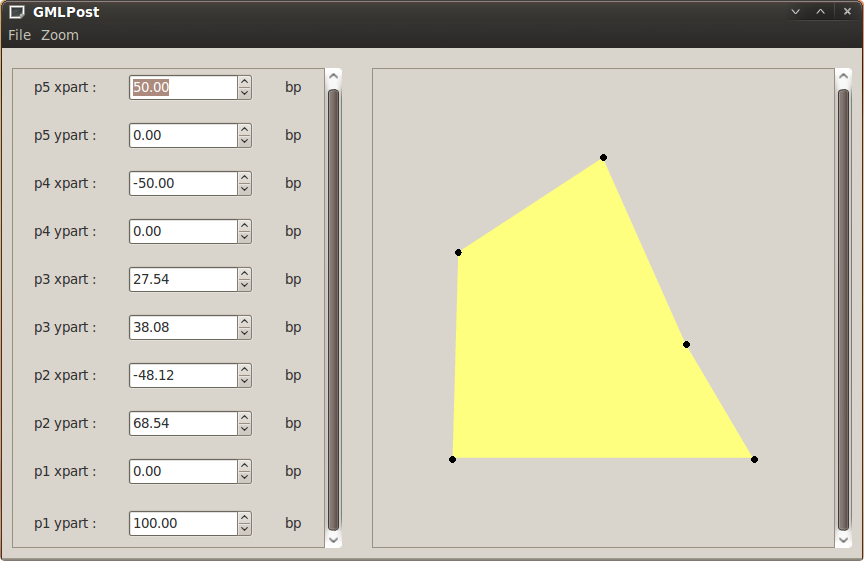
\includegraphics[scale=0.45]{screen1.png}

\begin{center}
\texttt{Exemple d'utilisation de \gmlpost\ avec 5 points éditables formant un polygone jaune} 
\end{center}

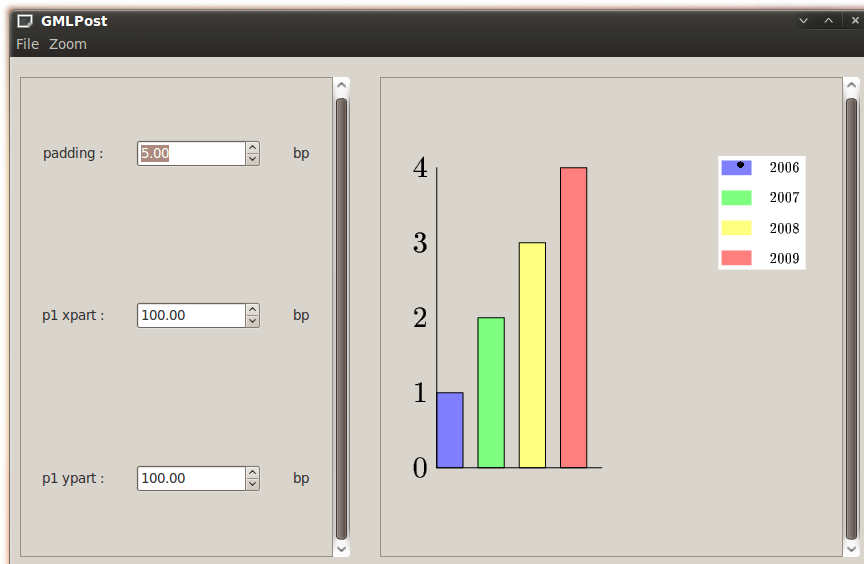
\includegraphics[scale=0.45]{screen2.png}

\begin{center}
\texttt{Exemple d'utilisation de \gmlpost\ avec un histogramme dont le padding est éditable et une légende dont la position est un point éditable } 
\end{center}

\section{Conclusion}
Les modules de ce TER ont tous été élaborés dans le but d'être ajoutés à \mlpost\ comme des modules \og haut niveau \fg\ à part entière. Nous avons respecté l'homogénéité de la bibliothèque au niveau des arguments optionnels (ex: dans tous les modules, \texttt{?fill} est l'argument remplissant l'élément de la couleur spécifiée), et au niveau de la documentation, rendant nos modules simples d'utilisation.

Nous avons effectué de nombreux tests pour nous assurer qu'après notre TER, les utilisateurs et les développeurs n'auraient pas à débugger. Le code est écrit assez proprement, et les fonctions récurcives sont terminales si possible.
Les modules sont opérationnels, mais peuvent ainsi être modifiés et complétés si nécessaire.

L'interface graphique n'a pu être terminée par faute de temps, et il demeure encore de nombreux aspects à travailler au niveau du canvas, du zoom, et de l'importation de figure.

Ce TER nous a permis de participer à l'élaboration à un stade avancé d'une bibliothèque de diagrammes, avec tout ce que cela implique de rigueur. Nous avons pu nous rendre compte en utilisant \texttt{lablgtk2} qu'une interface compliquée et pas claire rendait le travail beaucoup plus dur, ce qui rebutera à coup sûr les utilisateurs. Nous avons appris à utiliser les arguments optionnels fournis par \textsc{OCaml} et leurs subtilités, et nous sommes frottés à l'aspect object d'\textsc{OCaml}.

\begin{thebibliography}{99}
\bibitem{mlpost} \mlpost, une bibliothèque OCaml développée au sein du projet Proval de l’INRIA Saclay – Île-de-France, permettant la réalisation de dessins scientifiques destinés à être inclus dans des documents \LaTeX.

Auteurs:
\begin{itemize}
    \item Romain Bardou
    \item Johannes Kanig
    \item Stéphane Lescuyer
    \item Jean-Christophe Filliâtre 
\end{itemize}

\bibitem{tree}
Andrew Kennedy. 
\emph{Drawing Trees.}
Journal of Functional Programming, 
6(3): 527--534, Cambridge University Press, May 1996.
\end{thebibliography}

\end{document}

%%% Local Variables: 
%%% mode: latex
%%% mode: whizzytex
%%% mode: flyspell
%%% ispell-local-dictionary: "francais-latin1"
%%% End: 
